
%(BEGIN_QUESTION)
% Copyright 2008, Tony R. Kuphaldt, released under the Creative Commons Attribution License (v 1.0)
% This means you may do almost anything with this work of mine, so long as you give me proper credit

A piece of laboratory equipment uses a voltage divider to reduce voltage to two electromagnet coils from a higher-voltage source.  Coil \#1 is supposed to receive 2.91 volts and coil \#2 is supposed to receive 13.11 volts:

$$\includegraphics[width=15.5cm]{i03167x01.eps}$$

One day, something goes wrong with this circuit.  The magnetic field from coil \#1 suddenly becomes very weak, yet there is still a magnetic field coming from coil \#2.  The technician who looked at this problem before you took two voltage measurements and then gave up: 12.61 volts at test point TP3 and 41.7 millivolts at test point TP4.  You left your multimeter back at the shop, which means you cannot take any more voltage measurements.  However, since you are more determined than the former technician, you proceed to identify the following from the two measurements already taken:

\vskip 10pt

\begin{itemize}
\item{} \underbar{Two} components or wires in the circuit that you know cannot be failed either open or shorted, besides the 24 volt source which is obviously operational.
\vskip 40pt
\item{} \underbar{One} component or wire in the circuit you think could possibly be bad, and the type of failure it would be (either open or shorted).
\end{itemize}

\vfil 

\underbar{file i03167}
\eject
%(END_QUESTION)





%(BEGIN_ANSWER)

This is a graded question -- no answers or hints given!

%(END_ANSWER)





%(BEGIN_NOTES)

A good problem-solving technique is to first determine how much voltage {\it should} exist at test points TP3 and TP4 (both with respect to ground) if the circuit is healthy.  Doing the series-parallel analysis on this circuit shows that 13.11 volts are normally dropped across coil 2 ($V_{TP3}$), and 2.913 volts are normally dropped across coil 1 ($V_{TP4}$).

The only faults which could cause a slight decrease in coil 2 voltage while dramatically decreasing voltage at coil 1 would be a short-circuit across coil 1.  This would be a {\it real} short circuit (i.e. possessing some resistance), not a perfect short-circuit which of course would result in zero volts.

\vskip 10pt

\goodbreak
\noindent
{\bf Components known to be in good working condition:}

\begin{itemize}
\item{} Wire from battery to $R_1$
\item{} Wire from TP2 to TP3
\item{} $R_1$
\item{} $R_2$
\item{} Coil \#2
\end{itemize}

\vskip 10pt

\goodbreak
\noindent
{\bf Components which could possibly be faulted:}

\begin{itemize}
\item{} $R_3$ failed shorted
\item{} Coil \#1 failed shorted
\end{itemize}

%INDEX% Troubleshooting review: electric circuits

%(END_NOTES)


